\section{Máquinas de Turing}

\begin{frame}[fragile]{Funções efetivamente computáveis}

    \begin{block}{Definição}
        Uma função $f$ de inteiros positivos em inteiros positivos é \textbf{efetivamente 
        computável} se existe uma lista de instruções que, em princípio, permitam computar $f(n)$
        para qualquer argumento $n$.
    \end{block}

    \vspace{0.1in}

    \textbf{Observações}: a noção de computabilidade efetiva é intuitiva, pois não é rigorosamente
    definida. Contudo, as instruções da lista citada devem ser definidas e explícitas, de tal modo
    que possam ser seguidas sem exigir informações externas ou engenhosidade para a sua execução.
\end{frame}


\begin{frame}[fragile]{Máquina de Turing}

    \begin{block}{Definição}
        Uma \textbf{máquina de Turing} é uma máquina idealizada para realizar computação em 
        números inteiros positivos usando notação monádica (onde o inteiro positivo $n$ é 
        representado por $n$ traços). A computação acontece em uma finita linear, dividida em
        quadrados, infinita em ambas direções (esquerda e direita). Cada quadrado ou está 
        \textbf{em branco} (representado pelos símbolos $S_0, 0$ ou $\mathtt{B}$) ou tem 
        \textbf{um traço} ($S_1, 1$ ou $\mathtt{|}$).
        Exceto por um número finito de exceções, todos os demais quadrados estão em branco.
    \end{block}

    \vspace{0.1in}

    \textbf{Observações}: cada etapa da computação acontece em um quadrado da fita. O computador
    (agente humano, mecânico ou eletrônico) pode apagar o traço, caso o quadrado contenha um, ou 
    escrever um traço, caso o quadrado
    esteja vazio. Além disso, ele pode ser mover ou para o quadrado à esquerda, ou para o quadrado
    à direita.
\end{frame}

\begin{frame}[fragile]{Resumo das instruções possíveis para uma máquina de Turing}

    As instruções tem forma condicional, dizendo o que fazer caso o quadrado esteja em branco
    ($S_0$) ou contenha um traço ($S_1$):

    \vspace{0.1in}

    \begin{enumerate}[(1)]
        \item \textbf{Apagar:} escrever $S_0$ no quadrado, independente de seu estado
        \item \textbf{Escrever:} escrever $S_1$ no quadrado, independente de seu estado
        \item \textbf{Mover} para à esquerda ($R$)
        \item \textbf{Mover} para à direita ($L$)
        \item \textbf{Parar} a computação
    \end{enumerate}

    \vspace{0.1in}
    A instrução \textbf{(1)} em um quadrado em branco, ou a instrução \textbf{(2)} em um quadrado
    com um traço, equivalem a não fazer nada.
\end{frame}

\begin{frame}[fragile]{Estados e programa}

    \begin{itemize}
        \item Em cada etapa da computação, o computador avalia um quadrado em particular da fita

        \item O \textbf{estado} atual da máquina determina qual instrução (ação) a ser realizada
            e qual será o próximo estado que a 
            máquina assumirá, a depender se há um traço ou não no quadrado em avaliação

        \item Assim, cada etapa da computação depende do estado atual e do símbolo contido no 
            quadrado a ser avaliado

        \item Em cada etapa é realizada uma das cinco instruções listadas anteriormente, e é 
            determinado o próximo estado que a máquina assumirá

        \item Um \textbf{programa} consiste na descrição de todos os estados possíveis da máquina,
            e de todas as ações a serem seguidas em cada estado, a depender dos símbolos 
            encontrados no quadrado a ser avaliado
    \end{itemize}

\end{frame}

\begin{frame}[fragile]{Tabela de Máquina}

    \begin{block}{Definição}
        Uma \textbf{tabela de máquina} é uma tabela bidimensional cujas linhas representam
        os possíveis estados da máquina de Turing, e as duas colunas representam os símbolos 
        que podem estar escritos no quadrado a ser avaliado ($S_0$ ou $S_1$). Cada célula 
        descreve a ação a ser realizada, a depender do símbolo escrito, seguida do estado que 
        sucederá o estado atual.
    \end{block}

    \vspace{0.1in}

    Em uma fita inicialmente como todos os quadrados em branco, o programa abaixo escreve
    três traços consecutivos, e para.

    \begin{table}[h]
        \centering

        \begin{tabular}{c|cc}
            & $S_0$ & $S_1$ \\
            \hline
            $q_1$ & $S_1q_1$ & $Lq_2$ \\
            $q_2$ & $S_1q_2$ & $Lq_3$ \\
            $q_3$ & $S_1q_3$ \\
        \end{tabular}
    \end{table}
\end{frame}

\begin{frame}[fragile]{Fluxograma}

    \begin{block}{Fluxograma}
        Em um programa escrito em \textbf{fluxograma} cada estado possível da máquina é 
        representado por um círculo, e as transições possíveis são representadas por setas
        que partem do estado atual para o próximo estado, 
        com rótulos na forma $S_i:I_k$, onde $S_i$ é o símbolo presente no quadrado a ser
        avaliado e $I_k$ é a instrução a ser seguida.
    \end{block}

    \vspace{0.1in}

    Mesmo programa apresentado na tabela de máquina. A menos que indicado de outra maneira, é 
    assumido que a máquina inicia a computação no estado de menor número.

    \vspace{0.1in}

    \begin{figure}[h]
        \centering
        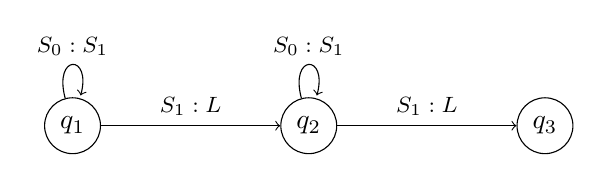
\begin{tikzpicture}
            \node[draw,circle] (q1) at (0, 0) { $q_1$ };
            \node[draw,circle] (q2) at (3, 0) { $q_2$ };
            \node[draw,circle] (q3) at (6, 0) { $q_3$ };

            \draw[->] (q1) edge node[anchor=south] { \footnotesize $S_1 : L$ } (q2);
            \draw[->] (q2) edge node[anchor=south] { \footnotesize $S_1 : L$ } (q3);
            \draw[->] (q1) edge[loop above] node[anchor=south] { \footnotesize $S_0 : S_1$ } (q1);
            \draw[->] (q2) edge[loop above] node[anchor=south] { \footnotesize $S_0 : S_1$ } (q2);

        \end{tikzpicture}
    \end{figure}

\end{frame}

\begin{frame}[fragile]{Conjunto de Quádruplas}

    \begin{block}{Definição}
        Um programa pode ser descrito por um conjunto de \textbf{quádruplas} 
        $(q_a, S_i, I_k, q_b)$, onde $q_a$ é o estado atual, $S_i$ o símbolo escrito no quadrado
        a ser avaliado, $I_k$ é a instrução (ação) a ser seguida e $q_b$ é o próximo estado.
        Se não houver ambiguidade, a quádrupla pode ser notada sem parêntesis e vírgulas, isto é,
        $q_aS_iI_kq_b$.
    \end{block}

    \vspace{0.1in}

    O programa ilustrado anteriormente por meio de tabela de máquina e de fluxograma, em lista 
    de quádruplas:
    \[
        q_1S_0S_1q_1,\ q_1S_1Lq_2,\
        q_2S_0S_1q_2,\ q_2S_1Lq_3,\
        q_3S_0S_1q_3
    \]
\end{frame}

\begin{frame}[fragile]{Configurações}

    \begin{itemize}
        \item O funcionamento de uma máquina de Turing pode ser descrito por meio de uma
            sequência de \textbf{configurações}

        \item Cada configuração lista todos os símbolos escritos na fita, o estado atual e 
            o quadrado a ser examinado

        \item Por exemplo, a configuração
        \[
            11010_3101
        \]
        representa uma fita com dois traços, um espaço em branco, um novo traço, um quadrado
        em branco, que está sendo examinado pelo estado $3$, um traço, um espaço em branco e 
        um traço

        \item Assume-se que os quadrados não listados contém, todos, espaços em branco

        \item Assim, o estado descrito acima seria idêntico as estados
            $011010_3101$ e $11010_310100$, por exemplo
    \end{itemize}

\end{frame}
